In our era technology has a foundamental role in almost every field. From the simple communications activities to those related to medical researches, technology is something we cannot do without. It is also a great opportunity in educational field, where it is demonstrated that the so called "stealth learning" (i.e. the help of technologies in educational scope) \cite{Sharp} is a solution to create a greater emotional involvement and that has as a consequence the ability to increase learner's learning opportunities. In our specific case, stealth learning is suitable for the treatment of patients affected by NDD to develop their cognitive, emotional and intellectual skills.

\section{Modern technologies for NDD people}
All the new existing technologies are now helping therapists and families to deal with neurological disabilities. In fact, in addition to virtual reality, smart objects, multisensor environments or smart spaces and conversational agents are used.\\
Smart objects are devices that can interact not only with the user but also with other similar devices and with the surrounding environment. Physical world can be described in terms of three properties \cite{Smart}: awareness (is a smart object to be able to understand events and human activities occurring in the physical world), representation (refers to a smart object's application and programming model) and interaction (denotes the object's ability to converse with the user in terms of input, output, control, and feedback).\\
Examples are Dolphin Sam \cite{Dolphin} and  Huggable \cite{Huggable}. \\
Smart spaces or multisensor environments are rooms in which children can play or interact in a controlled way because they are equipped with techonological items like cameras, smart objects, leds and projectors.
\\
Examples are Magic K room e M4All \cite{M4all}. \\
Conversational agents are devices that can communicate with the user in a manner consistent with what is required: an interaction of the user is answered by the agent who must be with sense.\\
\begin{figure}[H]
\centering
\begin{minipage}[c]{.40\textwidth}
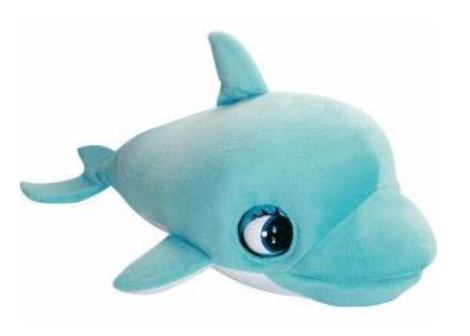
\includegraphics[width=1\textwidth]{immagini/delfino.png}
\end{minipage}%
\hspace{10mm}%
\begin{minipage}[c]{.40\textwidth}
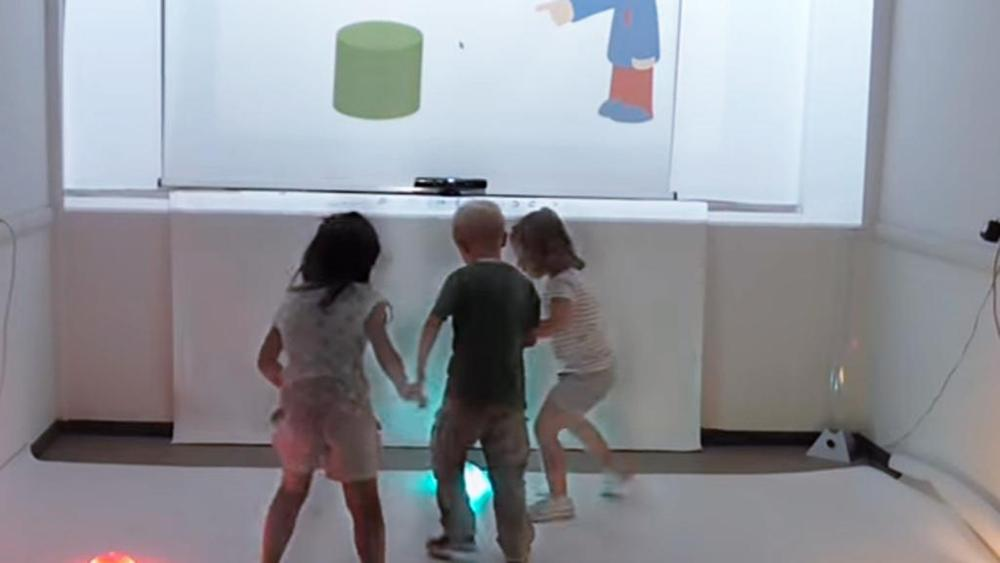
\includegraphics[width=1\textwidth]{immagini/stanzamagica.jpg}
\end{minipage}
\caption{Dolphin Sam and Magic K Room}\label{fig:smartimages}
\end{figure}

\section{Virtual Reality}
The great benefits of using Virtual Reality in an educational and rehabilitation context are now recognized worldwide and tested through various comparative tests between rehabilitation with the use of new technologies and rehabilitation with the use of classical methods \cite{Parsons}, \cite{Reid}, \cite{Wii}. In \cite{Pelagia} a review is carried out on recent literature to support and demonstrate the effectiveness of the use of VR with autistic children and in \cite{Tandra} the effects of a virtual reality game are analyzed to demonstrate the increase in social and emotional activities on a sample of 30 children between 7 and 16 years who suffer from ASD.\\
As previously mentioned, for the development of GEA, an approach that uses Werable Immersive Virtual Reality (WIVR) has been preferred since the possibility of a complete immersion in the environment and the removal of many distractions are the basis of an effective therapy. The user is in a world similar to the real one but safer as there is nothing that can hinder his learning and is reduced to the maximum the "fear" of making mistakes: it is as if the person could "train" the daily life so you can be ready and not catapulted into a world difficult for him. The use of the viewer also allows you to maintain a greater level of concentration because the player can not distract looking elsewhere or perceive the looks and reactions of those around, the only source of disturbance will then be sound. Once this type of games was not accessible to everyone because of the costs of technology and the problems that have been encountered in using it, such as a sense of nausea as sutied by the United States Army in \cite{Eugenia}, but nowadays many steps have been taken and viewers, as well as virtual reality itself, are within everyone's reach.\\
Regarding the technology of Virtual Reality viewers, HMDs, now on the market there is a clear division between two currents: embedded viewers, such as HTC Vive Pro, \cite{Vive}, and modular viewers, such as Google Cardboard, \cite{Cardboard}, and Samsung Gear VR, \cite{Gear}.\\
\textbf{HTC Vive Pro}
\begin{figure}[H]
\centering
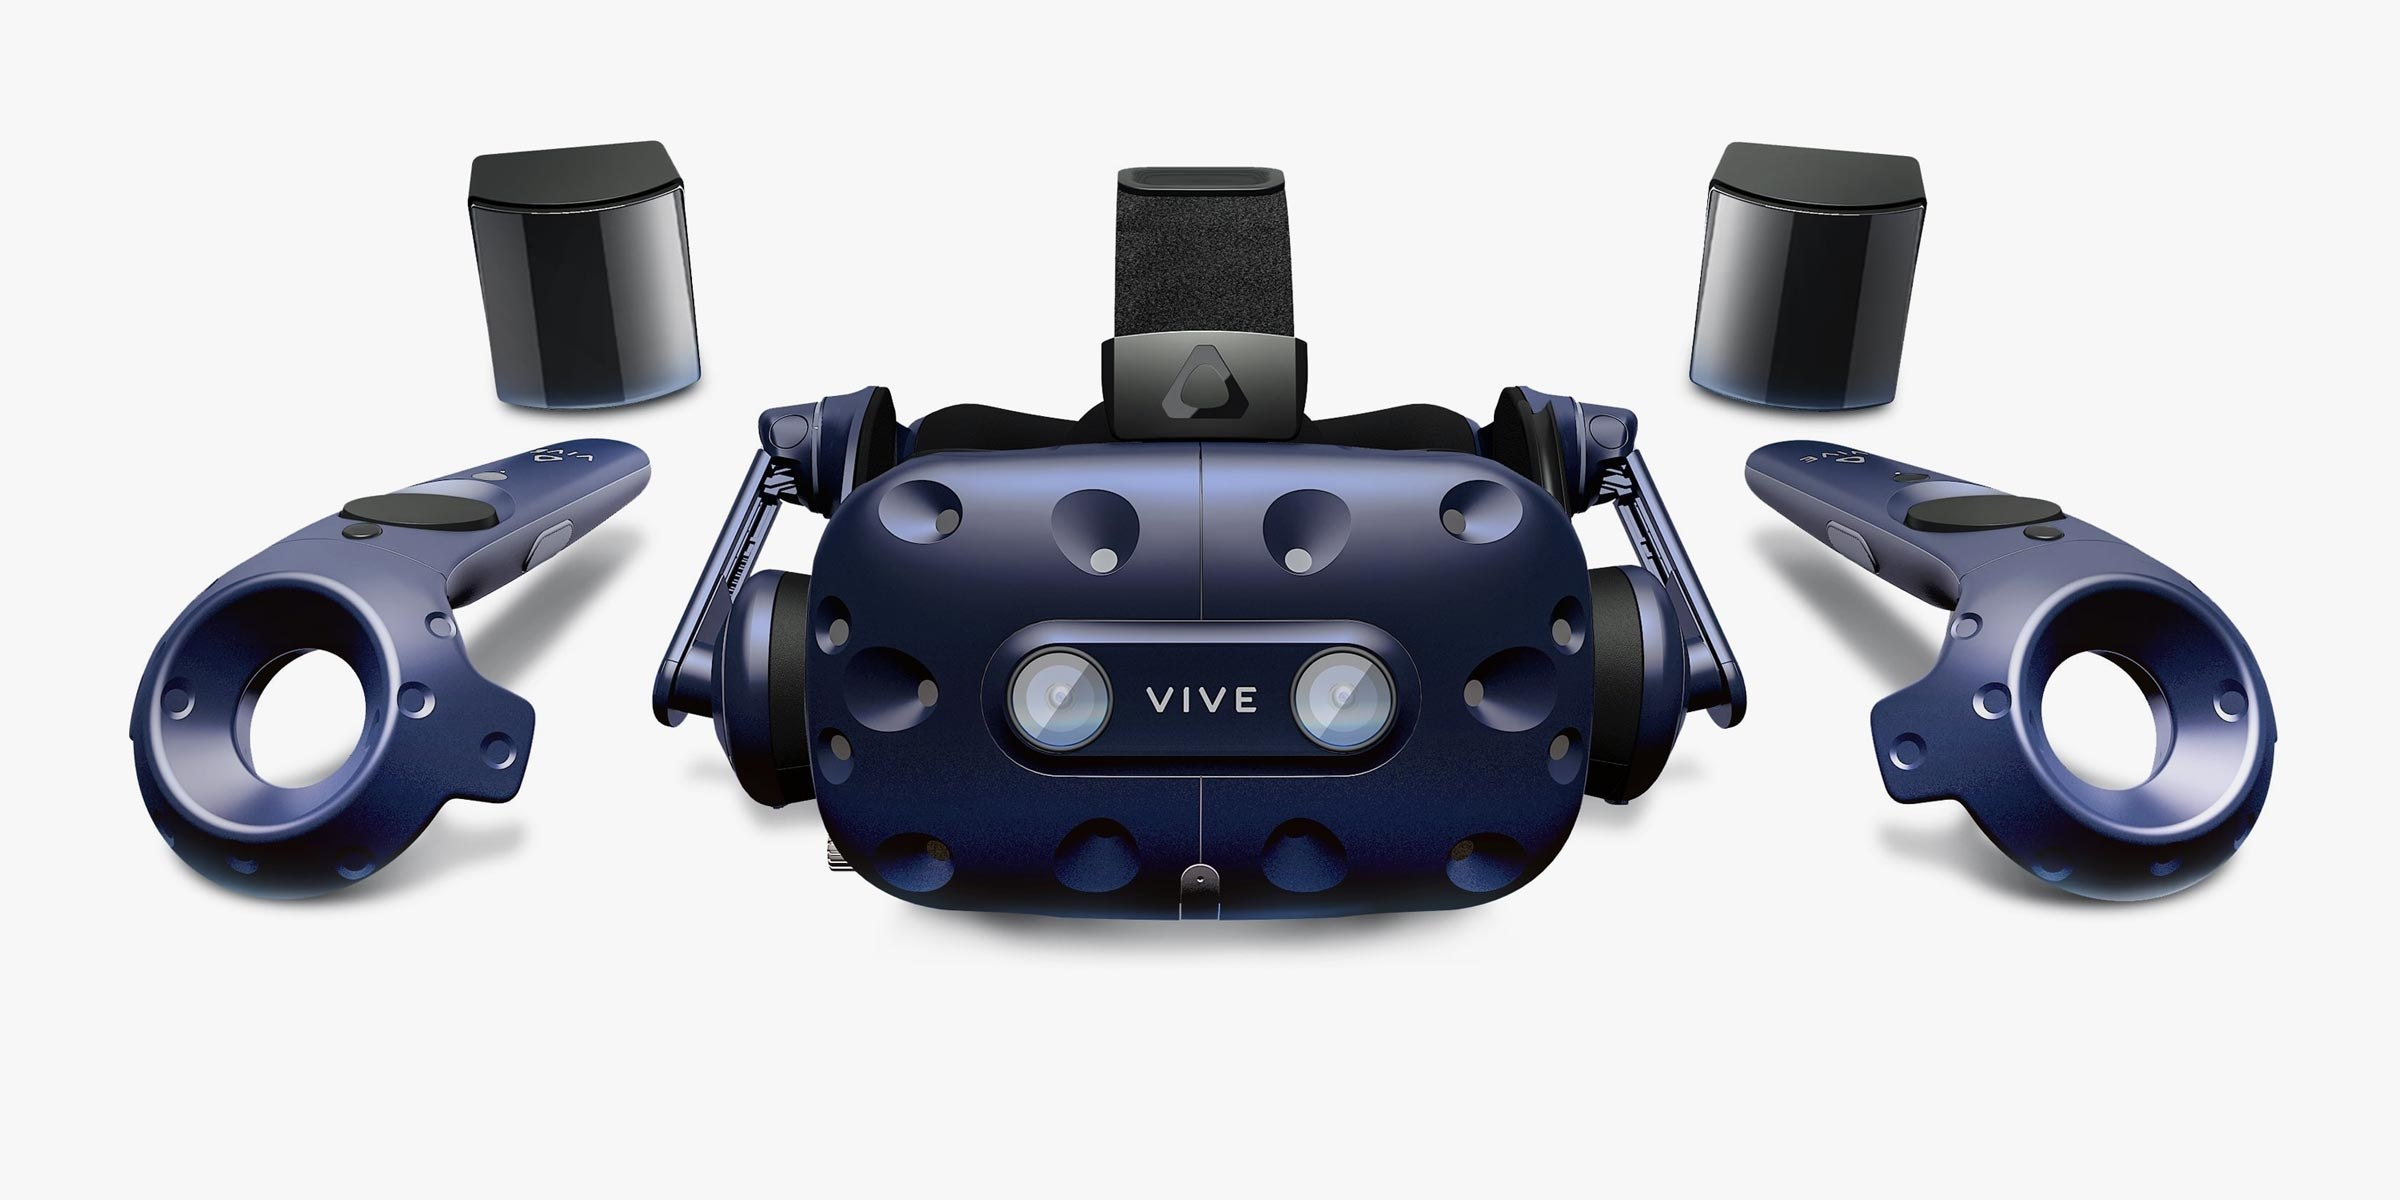
\includegraphics[width=12cm, height=6cm]{immagini/vive.jpg}
\caption{HTC Vive Pro}\label{fig:htcvive}
\end{figure}
HTC Vive Pro is an advanced virtual reality headset developed by HTC and Valve Corporation.The Vive Pro uses two screens, one per eye, each having a display resolution of 1440x1660. The displays are made of AMOLED technology, having a refresh rate of 90 Hz (90 frames per second). The device uses these sensors: SteamVr Tracking, G-Sensor, gyroscope, proximity and IPD sensor. It uses optimized ergonomics and lenses with 110 degrees. But it has a very high cost: 879 euro only the visor and 1399 euro the complete pack (from the official store).\\
\\
\textbf{Google Cardboard}
\begin{figure}[H]
\centering
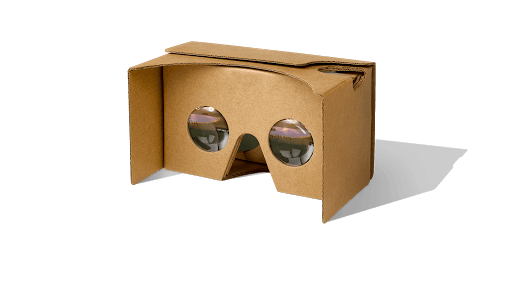
\includegraphics[width=12cm, height=6cm]{immagini/cardboard.png}
\caption{Google Cardboard}\label{fig:cardboard}
\end{figure}
Google Cardboard is composed of two biconvex lenses mounted on a plastic or cardboard frame available in different colors and shapes. The smartphone placed inside this structure shows the visual contents, subdividing them into two-dimensional images with two identical dimensions, and the interaction is obtained through the focused gaze. The user can navigate the virtual world by rotating his head which will consequently rotate the virtual scene projected on the display.\\
\\
\textbf{Samsung Gear VR}
\begin{figure}[H]
\centering
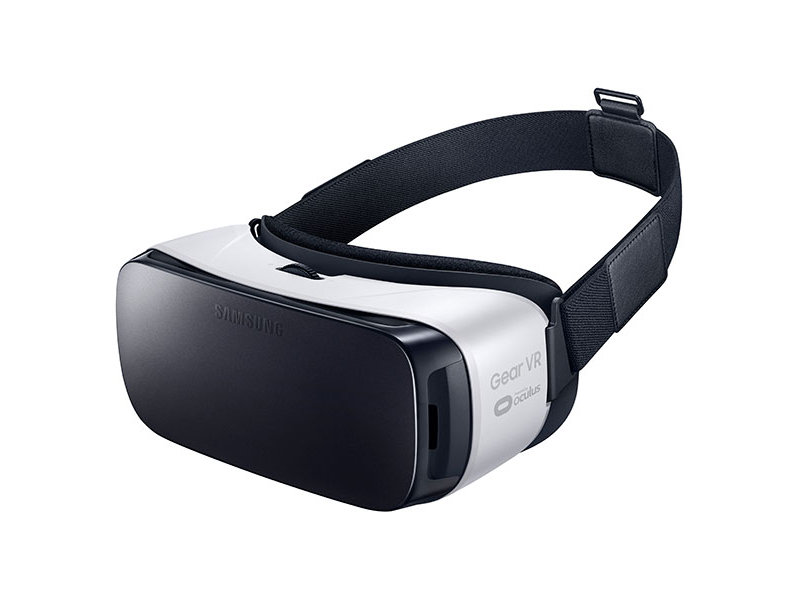
\includegraphics[width=10cm, height=6cm]{immagini/gear.jpg}
\caption{Samsung Gear VR}\label{fig:gearvr}
\end{figure}
Samsung Gear VR is still a modular HMD, produced by Samsung and Oculus VR. It is lightweight and with a good quality of materials,it has accelerometer, gyroscope and proximity Sensor but we can use it only with Samsung smartphones with some specifics. It costs more than Cardboard but it is not so expensive.\\
\\
During the implementation and testing phases of GEA we decided to use the modular visor as it turns out to be the most economical choice on the market and the financial factor is of great importance since the game is designed to be integrated into existing and widely adopted in therapeutic programs.

\section{Touchscreen}
The massive evolution that touchscreen devices have had in recent years, has strongly influenced our way of life. The amount of time a person spend on internet or on electronic devices in general is something that continues to grow every year. From a general point of view this is surely not a good thing because it has a large number of consequences that we have to take care of. \\
This new trend of life surely influences also children, that spend a lot of their time playing games on touchscreen devices, that are more accessible than traditional computers and video games because the motor skills needed to use them are not necessary.\\
\begin{figure}[H]
\centering
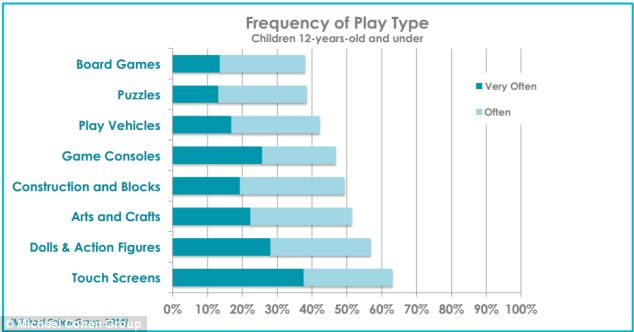
\includegraphics[width=10cm, height=7cm]{immagini/touch.png}
\caption{Time spent by children at playing games}\label{fig:timegames}
\end{figure}
Despite this kind of behaviour is largely criticized and not recommended by doctors and psychologists, the experiment conducted by B. Huber, J. Tarasuik, M.N. Antoniou, C. Garrett, S.J. Bowe and J. Kaufman \cite{Huber} demonstrated that children could learn from touchscreen educational games and apply this knowledge on physical problems. In fact there're a lot of applications thought for this purpose that help children to develop memory, problem-solving and executive functioning skills that could then be applied to real-world problems. The experiment shows substantially that there's no difference in learning for children that use real objects from those who learn only on touchscreen application. In particular, as observed by M.J. Mayo \cite{Mayo}, games could involve children more easily due to the presence of images, animations and sounds. Moreover, they're particularly adept at dosing information delivery. On a touchscreen application it is easy to complicate things and to add visual elements as the difficulty increases, while mantaining the focus on a small area that avoid extraneous distractions, so these educational games seems to be effective in enhancing motivation and increasing children interest in subject matter that leads to more effective learning \cite{Annetta}. 

\section{Google Chromecast}
Google Chromecast, \cite{Chromecast}, is a support device that we need for our application in order to exploit all its functionalities. It is a device that allows to send audio and video streams from a screen to another, without any wire through a technology called Google Cast.
\begin{figure}[H]
\centering
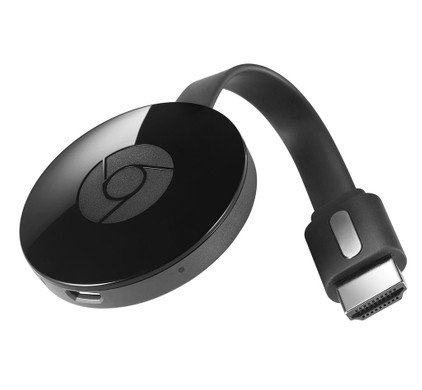
\includegraphics[width=7cm, height=6cm]{immagini/chromecast.jpg}
\caption{Google Chromecast}\label{fig:chromecast}
\end{figure}
In particular the link between the smartphone or tablet (what we want to replicate) and the Chromecast is done through a common wi-fi connection and Google Home app, then from the Chromecast to the television or computer (where we want to see the replication) through the direct connection of the key from the HDMI port. In this way we can replicate live contents and see what's going on inside the VR application or in the touchscreen one. \cite{Jared} \\
This technology, as said before, is essential for the purpose of our application, because we need it in order to allow group training and the possibility for the therapist to give explanation on what to do during the experience, that is one of the main feature of our application. 


\section{Projects about food education}
In the specific field of food education, we could find different kinds of game developed for touchscreen devices. In particular one example is the Food pyramid game developed by the Colorado State University \cite{Serrano} as a game to teach children what are the five main food groups and how to apply this knowledge to plan meal and snacks in order to increase their self-efficacy. This game is composed by various challenges regarding the food pyramid, and the researches has concluded that a game composed with a challenge is more effective that one based on a storyline.\\
Important companies are committed every year to the promotion and development of interactive educational games for children in this field both for the school and for the home, it is an example Nestl\'e with the project "Nutrikid", \cite{Nutrikid}, prepared with advice Scientific Committee of the NFI, Nutrition Foundation of Italy. As they read from their website "The Nutrition Foundation of Italy, was constituted legally as a non-profit association in December 1976, with the aim of activating interactions and collaborations with government bodies, universities and industry to contribute the development of scientific research, the exchange of information in the field of nutrition and the promotion of interdisciplinary research in this field.", \cite{NFI}, for this reason we have drawn great inspiration from it during the development of GEA. Other projects in this field are continually promoted by the FEI, Food Education Italy, a foundation of accredited participation at the Ministry of Education, University Research, which lives on voluntary contributions and is involved in helping schools and teachers to develop their role of food educators, \cite{FEI}.\\
Instead, as regards the specific field of food allergies, the state of the art appears to be scarce. It is possible to find, as applications, on the App Store and Play Store, only two games in this regard and both are in English, they are "Wizdy Diner" and "Allergy Reality" developed with touch screen technology and for PC. \cite{Wizdy} and \cite{Allergy}

\section{Participatory Design}
\subsection{What is Participatory Design?}
\subsection{Participatory Design with children}
\subsection{Participatory Design and people with disabilities}
